\documentclass[10pt,aspectratio=169]{beamer}    % 16/9

%----------------------------------------------------------------------------------------
%	PACKAGES AND THEMES
%----------------------------------------------------------------------------------------

\mode<presentation>{
  \usetheme{EuXFEL}
  \usecolortheme{EuXFEL}
}
\usepackage{hyperref}
\usepackage{amsmath}
\usepackage{graphicx}
\usepackage{subcaption}
\captionsetup[subfigure]{labelformat=simple,labelsep=colon}
\renewcommand{\thesubfigure}{}
\usepackage{helvet}
\usepackage[T1]{fontenc}
\usepackage{tikz}
\usepackage{ragged2e}
\usetikzlibrary{shapes, arrows, calc, positioning}
\usetikzlibrary{decorations.pathreplacing}
\usepackage{amsmath,amssymb}%,amsthm,amsxtra,mathabx}
\usepackage{mathtools, nccmath}
\usepackage{lipsum}
\usepackage{verbatim}
\usepackage{datetime}
\usepackage{listings}
\usepackage{animate}


\usepackage[backend=bibtex, sorting=ydnt]{biblatex}
\addbibresource{citation.bib}
\nocite{*}


\renewcommand{\familydefault}{\sfdefault}
\renewcommand\mathfamilydefault{}
\newcommand{\colorbf}[1]{{\color{xOrange}\textbf{#1}}}

\newdateformat{dmydate}{\monthname[\THEMONTH] \THEYEAR}   

\title[Integrasi Data Multisensor]{Integrasi Data Multisensor dan Sinkronisasi Waktu Pengukuran \\Untuk Melakukan Tracking Halangan dan Posisi Mobil Otonom}

\author{Adrian A. Firmansyah } % Your name
\institute[ITS] % Your institution as it will appear on the bottom of every slide, may be shorthand to save space
{\noindent
    adrianaryaputra@icloud.com\\
    6022201027\\
}

\date{\dmydate\today} % Date, can be changed to a custom date
\setbeamersize{text margin left=.05\pdfpagewidth,text margin right=.05\pdfpagewidth}
\setlength{\parskip}{1em}
\graphicspath{ {./src/img/} }



\begin{document}{
    \setbeamertemplate{headline}{}
    \begin{frame}
        \titlepage
    \end{frame}
}


\begin{frame}
    \Huge
    \begin{center}
        Kajian Pustaka
    \end{center}
\end{frame}


% KAJIAN PUSTAKA 1
\begin{frame}
    \begin{columns}
        \begin{column}{0.35\textwidth}
            \LARGE
            Kajian Pustaka 1
        \end{column}
        \begin{column}{0.6\textwidth}
            \justifying
            \textbf{Judul:}\\
            Extended Kalman Filter (EKF) design for vehicle position tracking using reliability function of Radar and Lidar

            \vspace{1.5em}

            \textbf{Penulis:}\\
            Kim, Taeklim; Park, Tae-Hyoung

            \vspace{1.5em}
            
            \textbf{Publikasi:}\\
            MDPI Sensors, vol.20, no.15, p.4126, 2020
        \end{column}
    \end{columns}
\end{frame}


\begin{frame}
    \frametitle{Pustaka 1: Pendahuluan}
    \large
    \begin{itemize}
        \justifying
        \item Desain Extended Kalman Filter untuk menggabungkan data Lidar dan Radar
        \vspace{1em}
        \item Menghasilkan algoritma yang mampu meningkatkan akurasi dibandingkan dengan hanya menggunakan satu macam sensor.
    \end{itemize}
\end{frame}


\begin{frame}
    \frametitle{Pustaka 1: Skema Sistem}
    \centering
    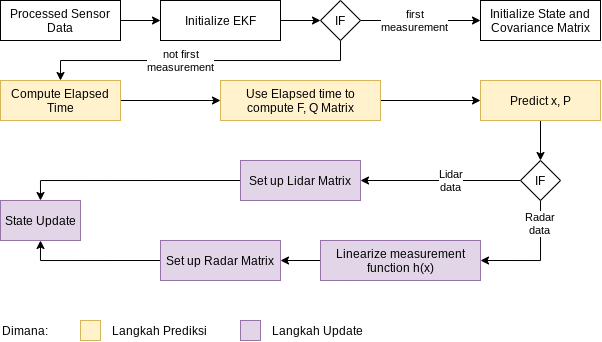
\includegraphics[width=.45\textwidth]{2-LREKF-diagram.png}
\end{frame}


\begin{frame}
    \frametitle{Pustaka 1: Metode}
    \begin{enumerate}
        \justifying
        \item pra-pemrosesan dilakukan menggunakan algoritma clustering dan asosiasi, dan menghasilkan centroid dari setiap objek halangan.
        \item Pada pengukuran pertama, inisialisasi state dan matriks kovarian 
        \item Prediksi dengan:
        \begin{itemize}
            \item Menghitung perubahan waktu
            \item Menghitung $F$ \& $Q$ baru berdasar perubahan waktu
            \item Prediksi $z$ \& $P$
        \end{itemize} 
        \item Bila data Radar, linearisasi fungsi pengukuran
        \item Update state dengan pengukuran dan $z$ baru.
        \item Tracking dengan hungarian Algorithm
    \end{enumerate}
\end{frame}


\begin{frame}
    \frametitle{Pustaka 1: Hasil}
    \centering
    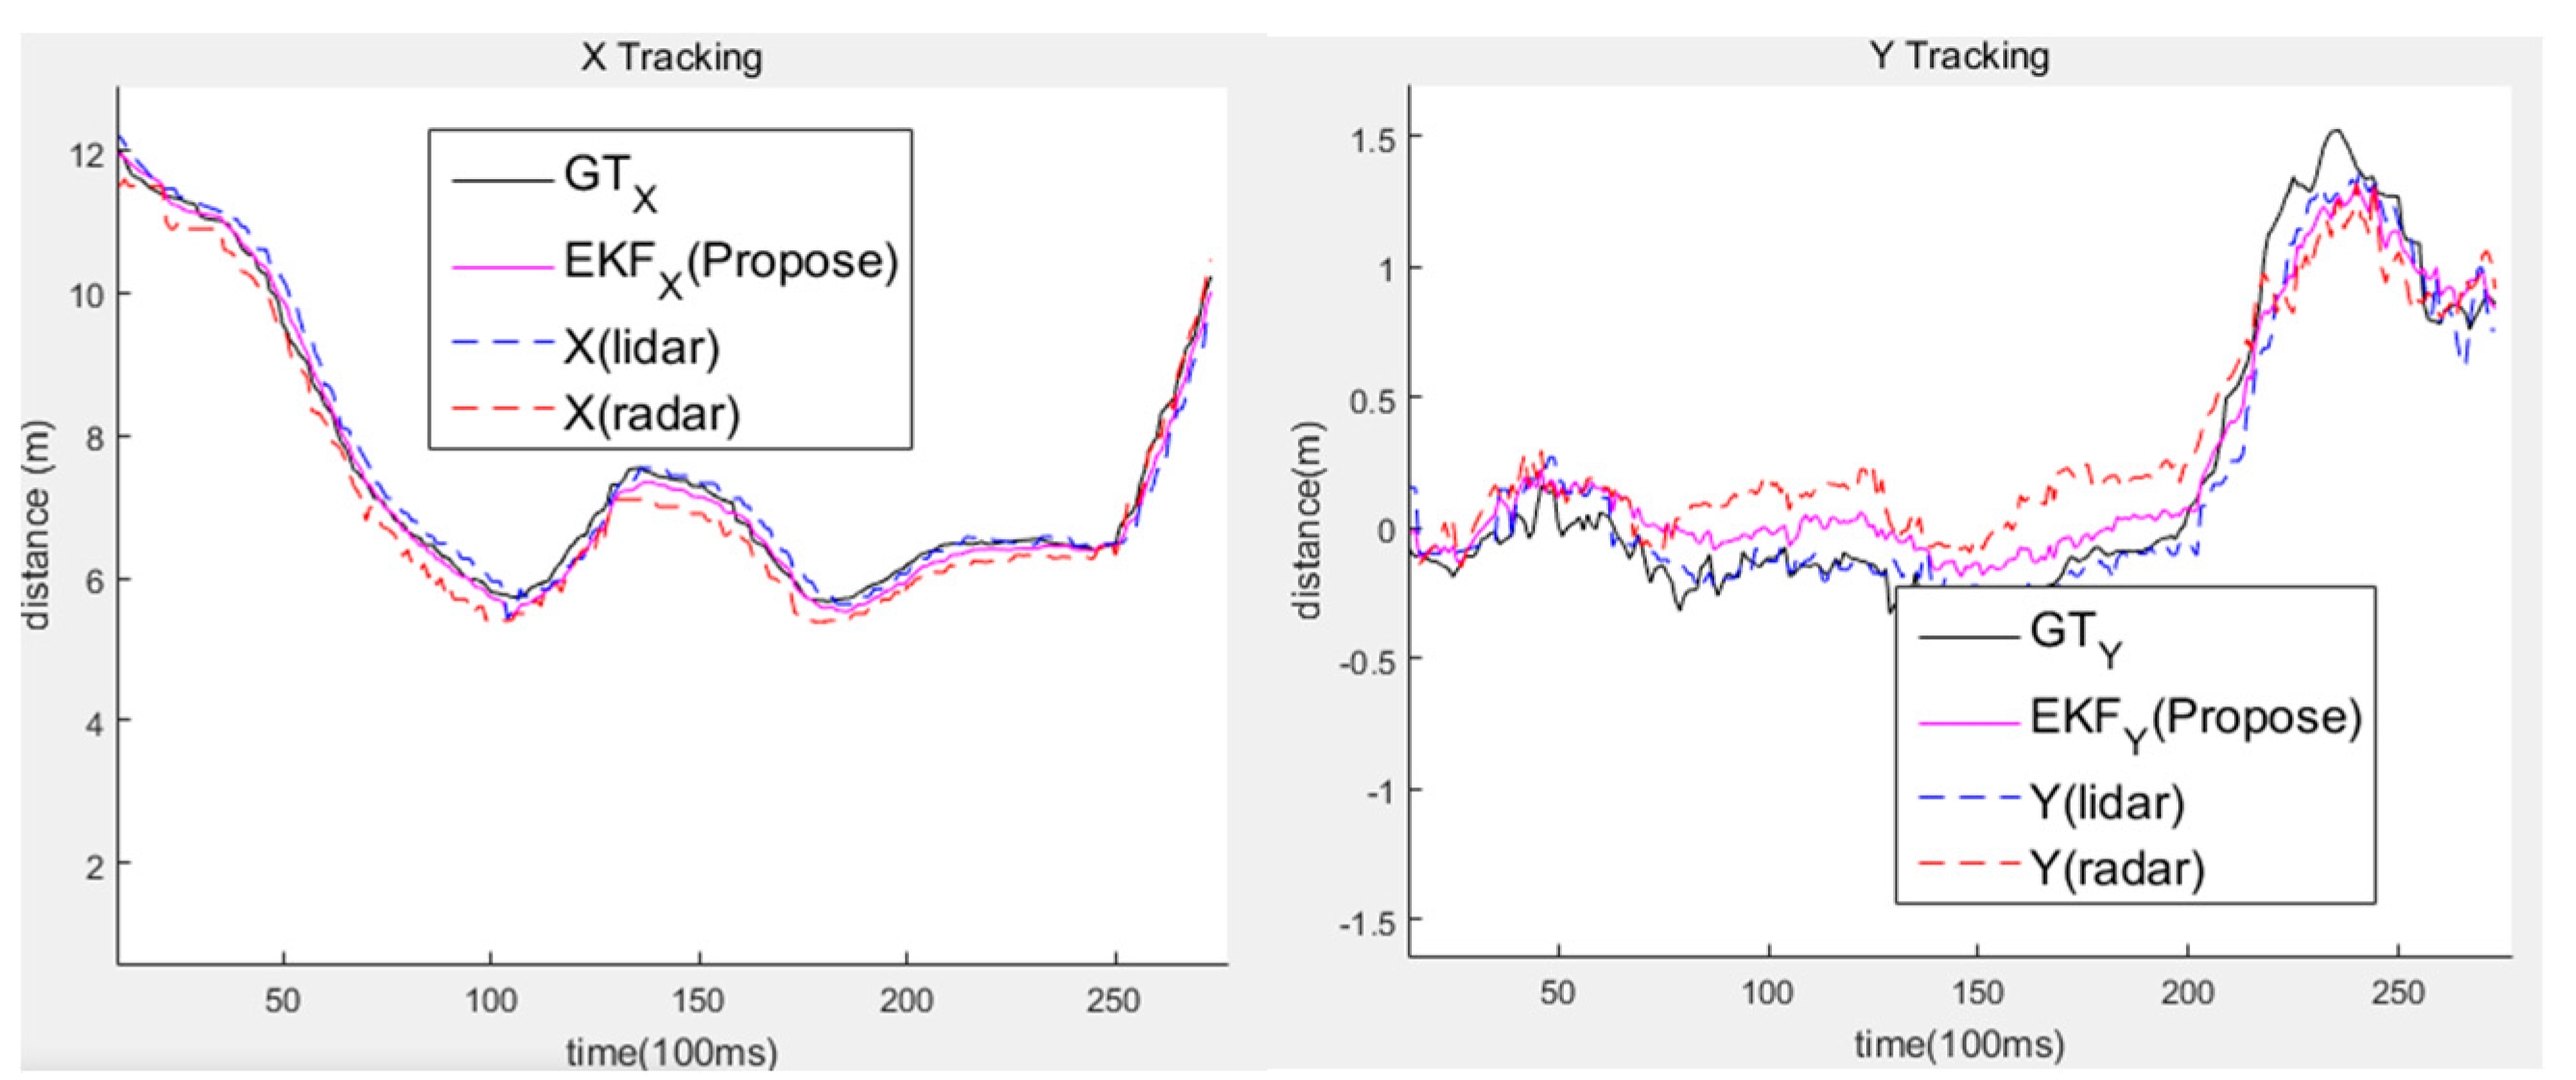
\includegraphics[width=.8\textwidth]{r1-hasil-1.png}
\end{frame}


\begin{frame}
    \frametitle{Pustaka 1: Hasil}
    \centering
    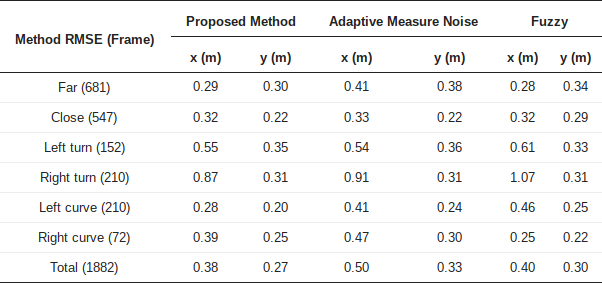
\includegraphics[width=.8\textwidth]{r1-hasil-2.png}
\end{frame}


\begin{frame}
    \frametitle{Pustaka 1: Kesimpulan}

    \large
    \textbf{Kelebihan}\\
    \normalsize
    \begin{itemize}
        \item Sensor Fusion Lidar dan Radar menggunakan algoritma ini lebih baik dibandingkan Adaptive Measure Noise dan Metode Fuzzy.
    \end{itemize}

    \large
    \textbf{Kekurangan}\\
    \normalsize
    \begin{itemize}
        \item Belum dapat membedakan jenis halangan karena hanya menggunakan Lidar dan Radar
        \item Penggunaan Lidar dan Radar redundant karena keduanya mengukur jarak.
    \end{itemize}

    \large
    \textbf{Ide}\\
    \normalsize
    \begin{itemize}
        \item Agar dapat membedakan jenis halangan, kamera dipilih untuk menggantikan radar karena mampu melakukan klasifikasi objek.
    \end{itemize}

\end{frame}

% KAJIAN PUSTAKA 2

\begin{frame}
    \begin{columns}
        \begin{column}{0.35\textwidth}
            \LARGE
            Kajian Pustaka 2
        \end{column}
        \begin{column}{0.6\textwidth}
            \justifying
            \textbf{Judul:}\\
            Spatial Attention fusion for obstacle detection using mmwave radar and vision sensor

            \vspace{1.5em}

            \textbf{Penulis:}\\
            Chang, Shuo; Zhang, Yifan; Zhang, Fan; Zhao, Xiaotong; Huang, Sai; Feng, Zhiyong; Wei, Zhiqing

            \vspace{1.5em}
            
            \textbf{Publikasi:}\\
            MDPI Sensors, vol.20, no.4, p.956, 2020
        \end{column}
    \end{columns}
\end{frame}


\begin{frame}
    \frametitle{Pustaka 2: Pendahuluan}
    \large
    \begin{itemize}
        \justifying
        \item mengintegrasikan Radar mmWave dengan Kamera untuk mendapatkan hasil deteksi halangan menggunakan metode Spatial Attention Feature (SAF)
        \vspace{1em}
        \item Mendapatkan hasil deteksi halangan yang lebih baik dibandingkan hanya menggunakan kamera atau radar
    \end{itemize}
\end{frame}


\begin{frame}
    \frametitle{Pustaka 2: Skema Sistem}
    \centering
        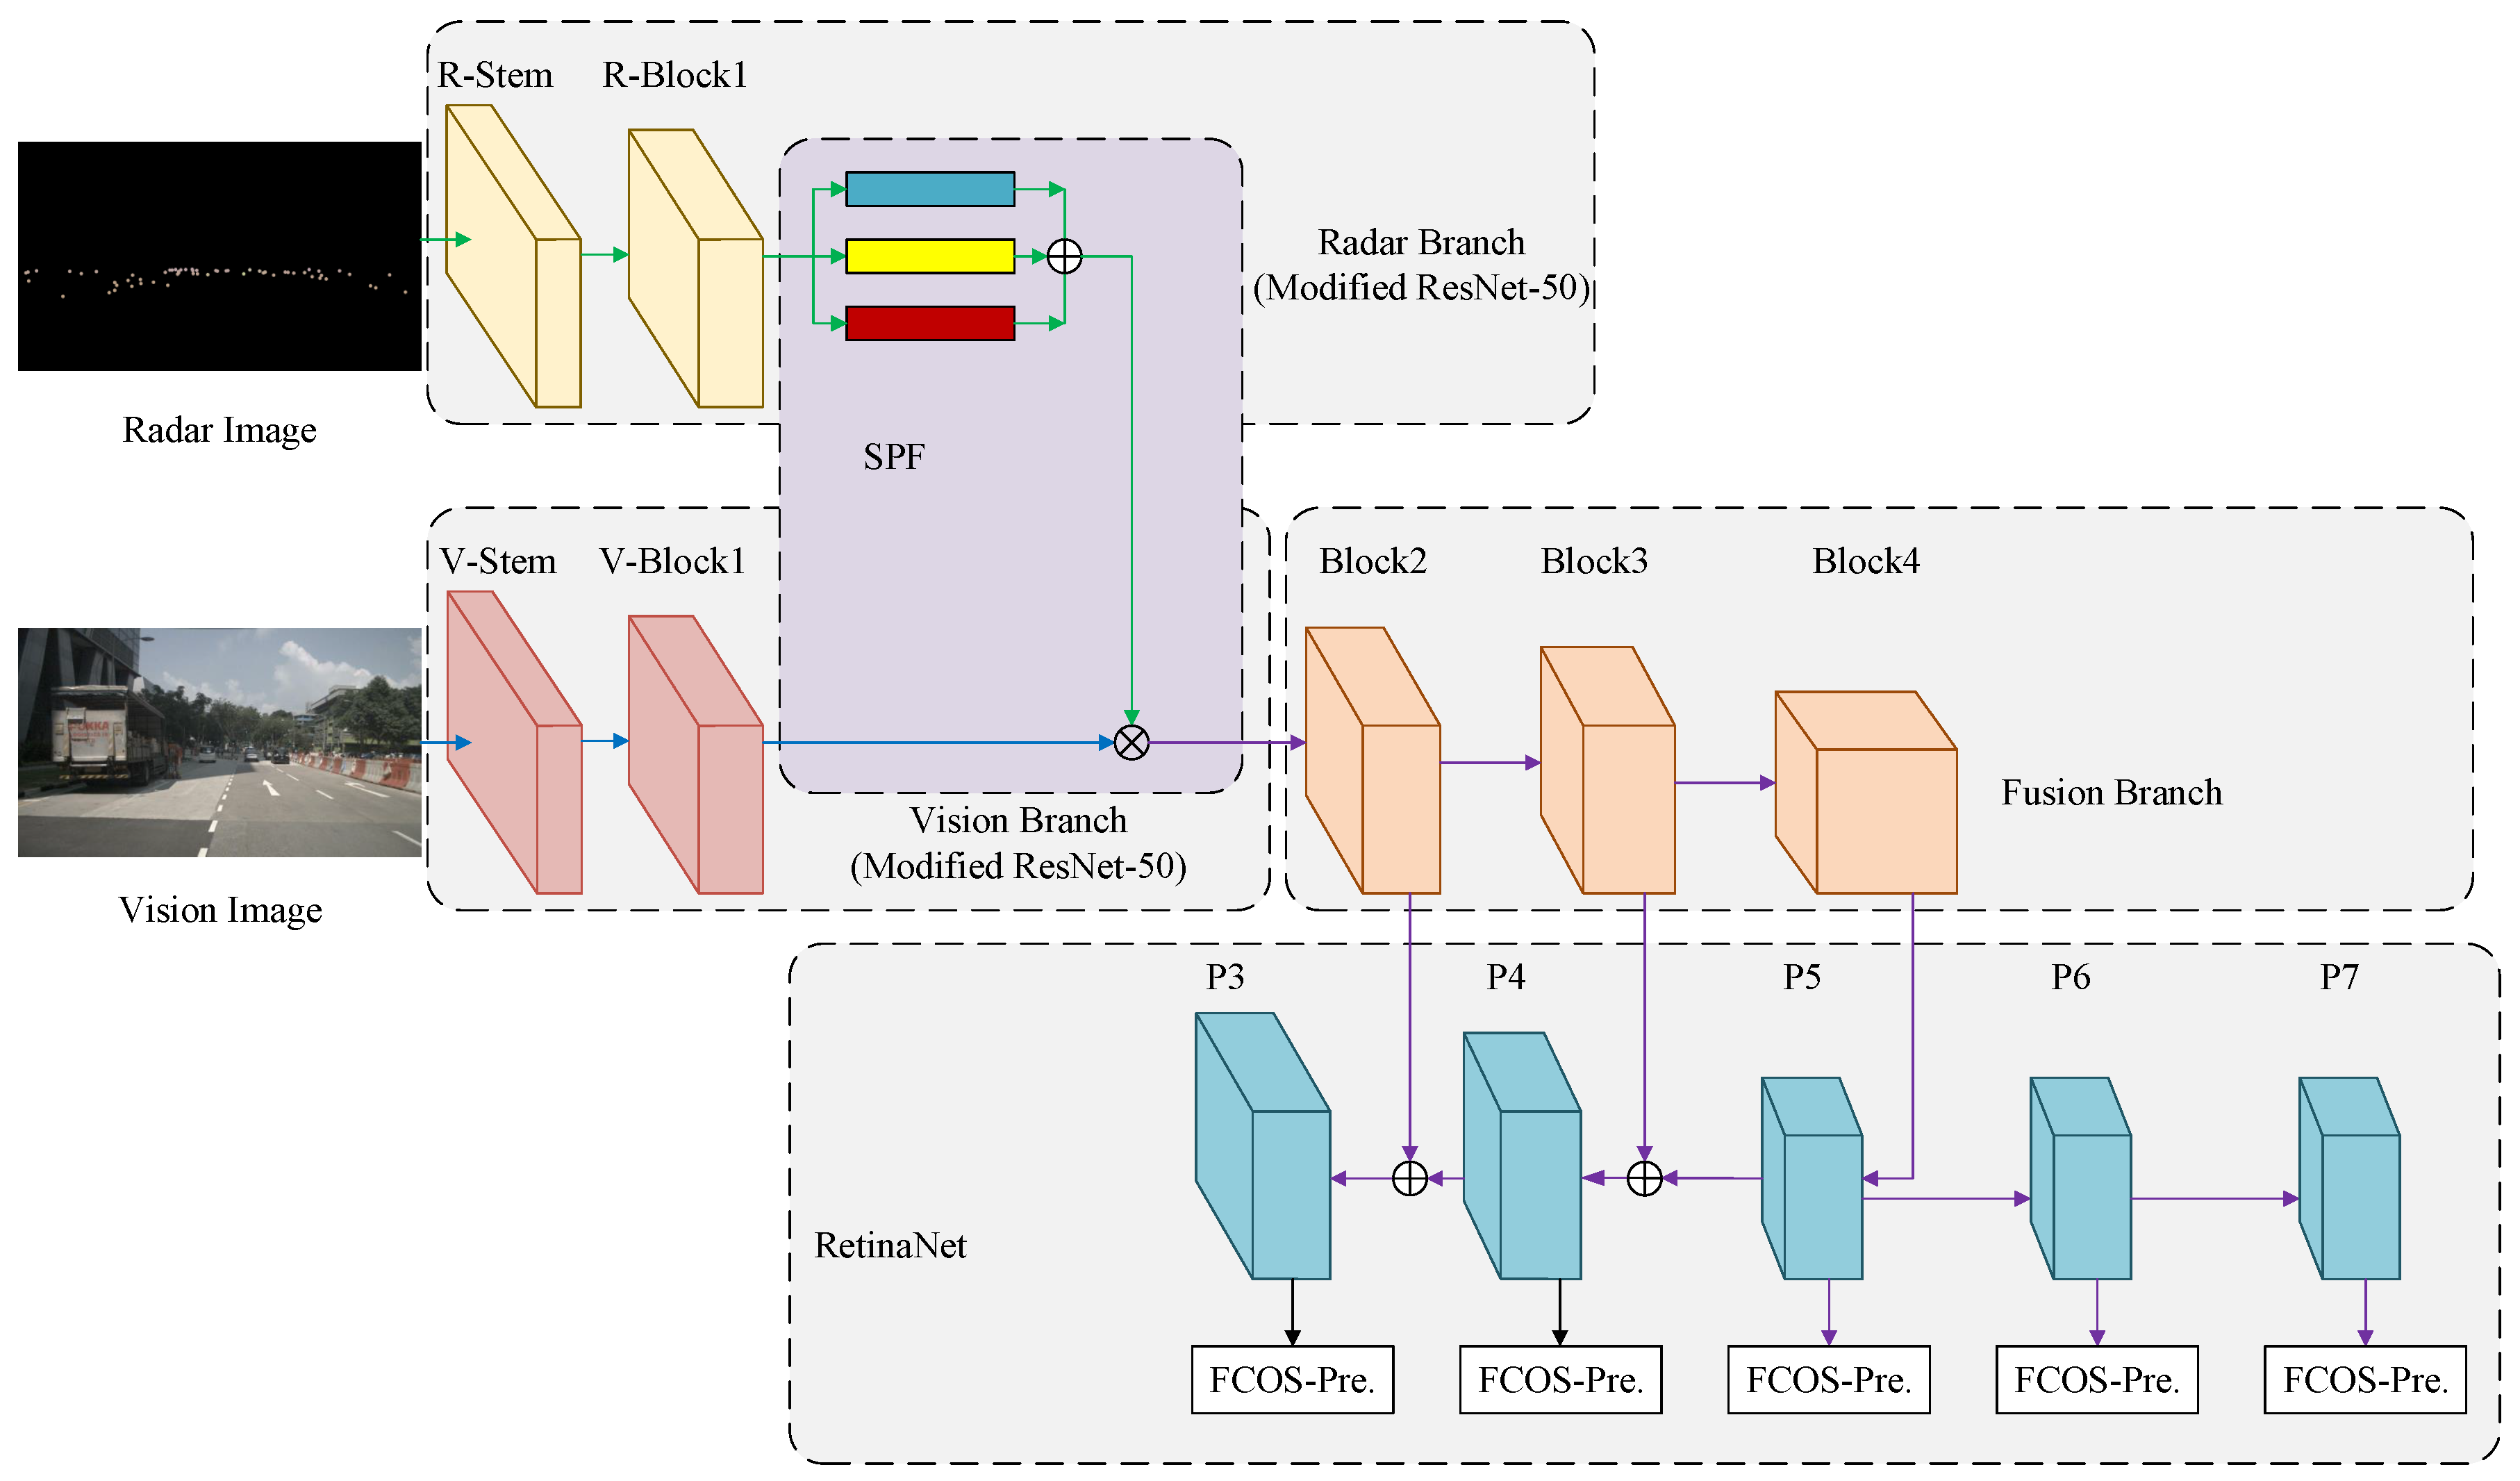
\includegraphics[width=.6\textwidth]{2-SAF-diagram.png}
\end{frame}


\begin{frame}
    \frametitle{Pustaka 2: Metode}
    \begin{enumerate}
        \justifying
        \item Deteksi Fitur Gambar dan Radar dengan ResNet50
        \item Fitur radar dimasukkan ke blok SAF/SPF
        \item Keluaran SAF dan Gambar digabungkan dengan Fusion Branch berbasis ResNet50
        \item Penentuan posisi dengan pyramid network RetinaNet
    \end{enumerate}
\end{frame}


\begin{frame}
    \frametitle{Pustaka 2: Hasil}
    \centering
    \includegraphics[width=\textwidth]{r2-hasil-1.png}
\end{frame}


\begin{frame}
    \frametitle{Pustaka 2: Hasil}
    \centering
    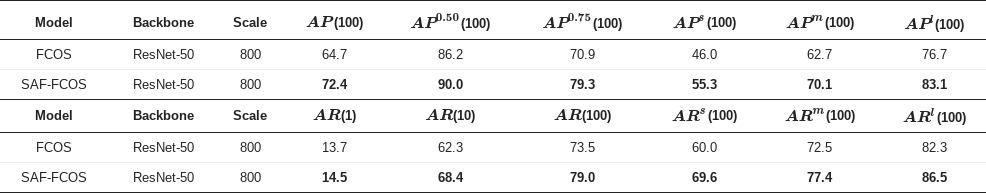
\includegraphics[width=\textwidth]{r2-hasil-2.png}
\end{frame}


\begin{frame}
    \frametitle{Pustaka 2: Kesimpulan}

    \large
    \textbf{Kelebihan}\\
    \normalsize
    \begin{itemize}
        \item Permodelan sistem lebih mudah karena fusion dilakukan di tingkat Fitur, tepat setelah ekstraksi fitur gambar dan radar.
    \end{itemize}

    \large
    \textbf{Kekurangan}\\
    \normalsize
    \begin{itemize}
        \item Permodelan di tingkat fitur menyebabkan Kamera dan Radar menjadi terkopel, sehingga keduanya harus bekerja dengan baik agar keluaran algoritma ini sesuai keinginan desain.
    \end{itemize}

    \large
    \textbf{Ide}\\
    \normalsize
    \begin{itemize}
        \item Metode deteksi gambar pada penelitian ini dapat digunakan sepenuhnya.
        \item Mencoba fusion di tingkat data.
        \item Menggunakan algoritma ini sebagai pembanding.
    \end{itemize}

\end{frame}

% KAJIAN PUSTAKA 3

\begin{frame}
    \begin{columns}
        \begin{column}{0.35\textwidth}
            \LARGE
            Kajian Pustaka 3
        \end{column}
        \begin{column}{0.6\textwidth}
            \justifying
            \textbf{Judul:}\\
            A novel hybrid fusion algorithm for low-cost GPS/INS integrated navigation system during GPS outages

            \vspace{1.5em}

            \textbf{Penulis:}\\
            Li, Dengao; Jia, Xuan; Zhao, Jumin

            \vspace{1.5em}
            
            \textbf{Publikasi:}\\
            IEEE Access, vol.8, p.53984-53996, 2020
        \end{column}
    \end{columns}
\end{frame}


\begin{frame}
    \frametitle{Pustaka 3: Pendahuluan}
    \large
    \begin{itemize}
        \justifying
        \item Metode hybrid GPS / INS yang diusulkan dapat mendeteksi posisi dengan tepat walaupun terdapat GPS outage dan menggunakan GPS berbiaya rendah.
        \vspace{1em}
        \item Menggunakan Extreme Learning Machine untuk memberikan estimasi error INS terhadap GPS pada saat GPS padam.
        \vspace{1em}
        \item Pada saat GPS menyala, data error GPS digunakan untuk melakukan training ELM
    \end{itemize}
\end{frame}


\begin{frame}
    \frametitle{Pustaka 3: Skema Sistem}
    \centering
    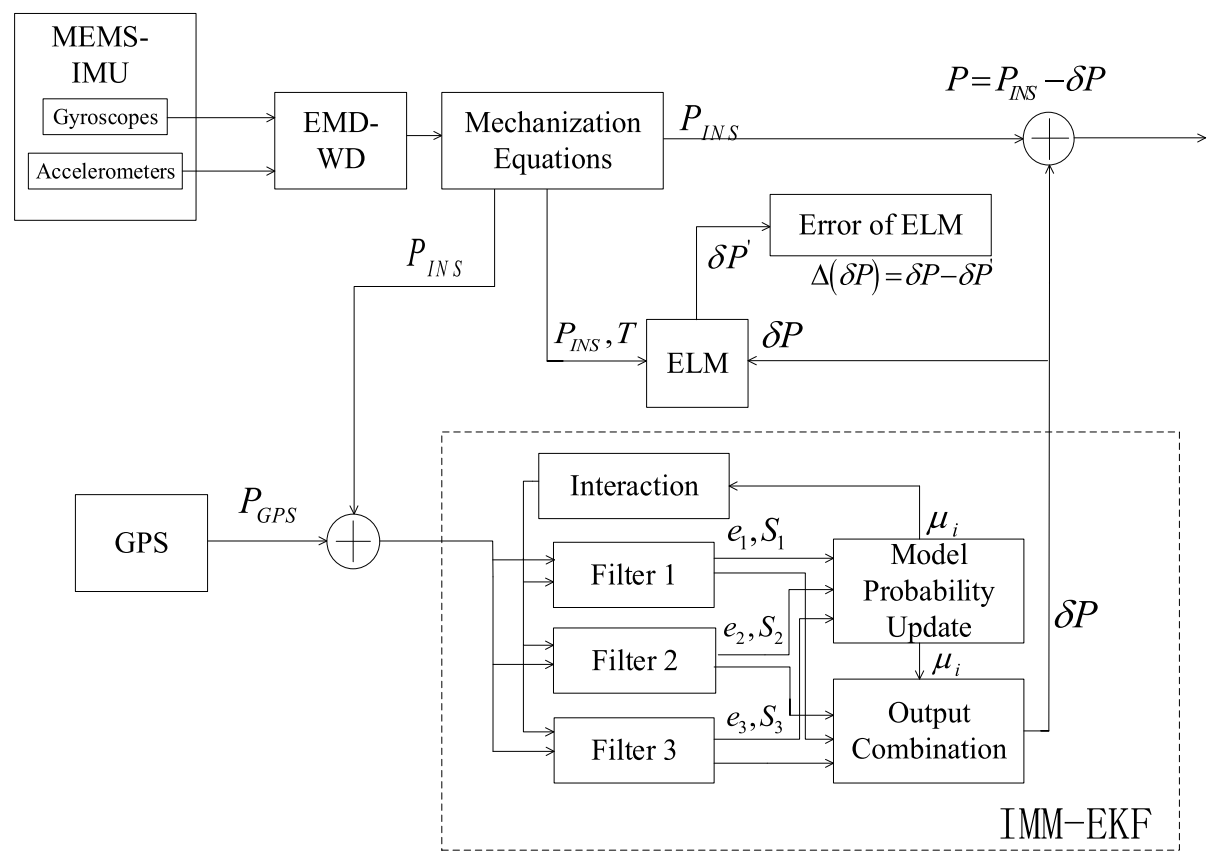
\includegraphics[width=.6\textwidth]{2-GPSINS-diagram.png}
\end{frame}


\begin{frame}[allowframebreaks]
    \frametitle{Pustaka 3: Metode. Bagian}
    \begin{enumerate}
        \justifying
        \item Hasil pembacaan INS difilter menggunakan Empirical Mode Decomposition Wavelet Denoising (EMD-WD).
        \vspace{1em}
        \item Hasil filter EMD-WD dimasukkan ke persamaan mekanisasi INS untuk mendapatkan posisi dan kecepatan.
        \vspace{1em}
        \item Posisi INS dan GPS dimasukkan ke Imterctive Multi-Model Kalman Filter (IMM-EKF) untuk mendapatkan error posisi untuk mengkoreksi INS.
        \vspace{1em}
        \pagebreak
        \item Apabila data GPS tersedia, Hasil persamaan mekanisasi INS, dan error posisi untuk koreksi INS yang dihasilkan IMM-EKF dijadikan sebagai data training untuk ELM.
        \vspace{1em}
        \item Apabila terjadi blackout, data keluaran IMM-EKF yang membutuhkan GPS diubah menjadi data keluaran ELM menggunakan masukkan dari persamaan mekanisasi INS.
    \end{enumerate}
\end{frame}


\begin{frame}
    \frametitle{Pustaka 3: Sistem saat blackout}
    \centering
    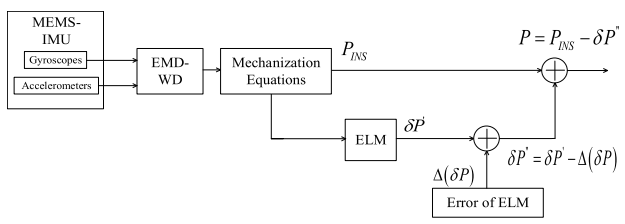
\includegraphics[width=.8\textwidth]{r3-prediksi.png}
\end{frame}


\begin{frame}
    \frametitle{Pustaka 3: EMD-WD}
    \centering
    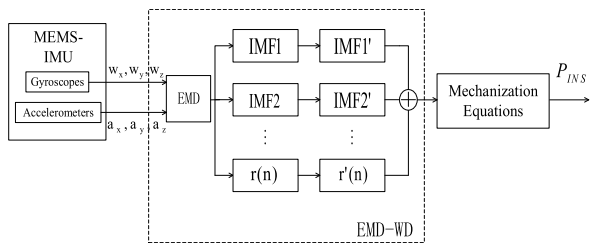
\includegraphics[width=.8\textwidth]{r3-EMDWD.png}
\end{frame}


\begin{frame}
    \frametitle{Pustaka 3: ELM}
    \centering
    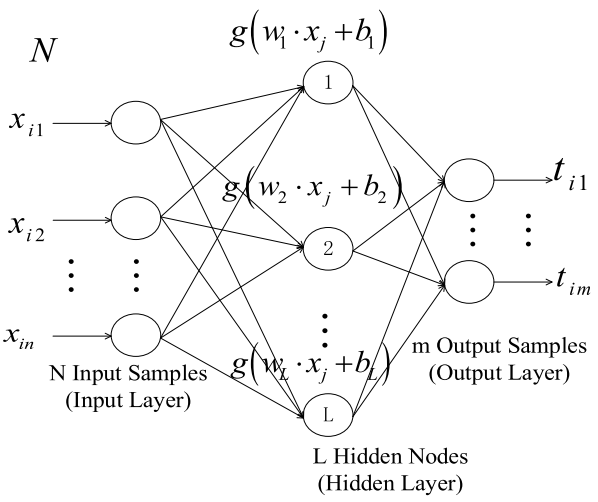
\includegraphics[width=.5\textwidth]{r3-ELM.png}
\end{frame}


\begin{frame}
    \frametitle{Pustaka 3: Hasil}
    \centering
    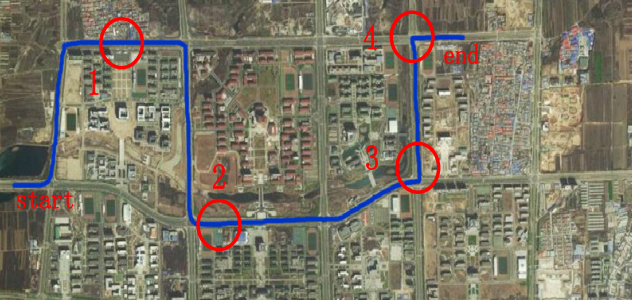
\includegraphics[width=.8\textwidth]{r3-hasil1.png}\\
    uji lapangan dengan lingkaran merah merupakan lokasi blackout GPS.
\end{frame}


\begin{frame}
    \frametitle{Pustaka 3: Hasil}
    \centering
    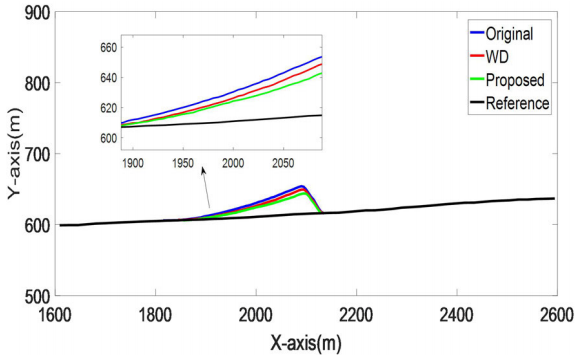
\includegraphics[width=.6\textwidth]{r3-hasil2.png}\\
    drift error pada wilayah uji 1
\end{frame}


\begin{frame}
    \frametitle{Pustaka 3: Kesimpulan}

    \large
    \textbf{Kelebihan}\\
    \normalsize
    \begin{itemize}
        \item Metode fusion hybrid INS dengan GPS pada penelitian ini dapat mengurangi drift error pada posisi INS saat tidak terdapat informasi dari GPS.
    \end{itemize}

    \large
    \textbf{Ide}\\
    \normalsize
    \begin{itemize}
        \item Algoritma fusi hybrid INS-GPS pada penelitian ini dapat digunakan sepenuhnya sebagai sub-sistem integrasi INS-GPS.
        \item posisi kendaraan yang dihasilkan oleh algoritma ini akan digunakan untuk mengubah posisi halangan yang dideteksi dari yang sebelumnya relatif terhadap kendaraan menjadi relatif terhadap bumi.
    \end{itemize}

\end{frame}



\begin{frame}
    \Huge
    \begin{center}
        Pendahuluan
    \end{center}
\end{frame}


\begin{frame}
    \frametitle{Rumusan Masalah}
    \begin{enumerate}
        \item Mobil otonom memerlukan sensor yang mampu menggantikan fungsi dan kemampuan dari indera manusia, terutama kemampuan untuk memperkirakan jarak halangan di sekitarnya.
        \item Lidar dapat menentukan jarak secara akurat, namun tidak dapat membedakan jenis dari halangan.
        \item Kamera dengan klasifikasi objek mampu membedakan jenis halangan, namun tidak dapat menentukan jarak secara akurat.
        \item Dibutuhkan metode untuk melakukan track pada halangan yang telah terdeteksi agar mobil dapat mengetahui halangan di sekitarnya.
        \item Waktu dan periode pengukuran dari setiap sensor berbeda-beda.
    \end{enumerate}
\end{frame}


\begin{frame}
    \frametitle{Tujuan}
    \justifying
    Tujuan dari penelitian ini adalah melakukan tracking halangan, posisi, dan pose kendaraan yang didapatkan melalui gabungan sensor Kamera, Lidar, GPS serta INS menggunakan Extended Kalman Filter Multi-Object Tracking pada data eksternal, dan Extended Kalman Filter (EKF) pada data internal dengan mempertimbangkan perbedaan waktu dan periode pengukuran tiap sensor sehingga hasil tracking menjadi lebih akurat dibandingkan dengan data yang dihasilkan oleh satu sensor tanpa mempertimbangkan perbedaan waktu pengambilan sampel deteksi.
\end{frame}


\begin{frame}
    \frametitle{Batasan Masalah}
    \justifying
    \begin{enumerate}
        \justifying
        \item Sensor deteksi jarak menggunakan Lidar.
        \item Rentang deteksi Lidar dibatasi pada kemampuan sensor yang dimiliki.
        \item Objek tracking terklasifikasi dibatasi pada mobil dan pedestrian, namun tidak menutup kemungkinan untuk dilakukan penambahan klasifikasi lainnya.
        \item Pengambilan data akan dilakukan secara nyata, namun tidak menutup kemungkinan akan digunakan simulasi menggunakan Microsoft AirSim apabila kemampuan deteksi sensor yang dibutuhkan tidak mencukupi.
    \end{enumerate}
\end{frame}


\begin{frame}
    \frametitle{Kontribusi}

    \justifying
    Kontribusi dari penelitian ini menghasilkan sistem tracking halangan, posisi, dan pose kendaraan yang didapatkan melalui gabungan sensor Kamera, Lidar, GPS, serta INS menggunakan Kalman filter dengan mempertimbangkan perbedaan waktu sampel setiap sensor sehingga hasil tracking menjadi lebih akurat dibandingkan dengan tanpa mempertimbangkan perbedaan waktu pengambilan sampel deteksi.


\end{frame}


\begin{frame}
    \Huge
    \begin{center}
        Metodologi Penelitian
    \end{center}
\end{frame}


\begin{frame}
    \frametitle{Skema Sistem yang diajukan}
    \begin{center}
        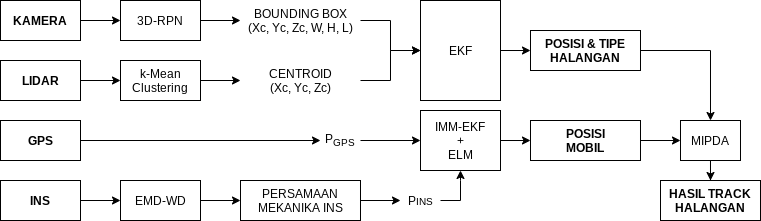
\includegraphics[width=\textwidth]{3-sistem.png}
    \end{center}
\end{frame}


\begin{frame}
    \frametitle{INS: Wavelet Denoising}
    EMD mendekomposisi sinyal x menjadi beberapa Instrinsic Mode Function (IMF). Hasil dekomposisi berbentuk jumlahan n komponen IMF dan sinyal residual. $c_n(t)$ merupakan komponen IMF, dan $r_n(t)$ merupakan sinyal residual
    \begin{equation}
        x(t)=\sum_{i=1}^{n} c_{i}(t)+r_{n}(t)
    \end{equation}
    Kemudian dilakukan wavelet denoising pada setiap komponen IMF, sehingga menghasilkan
    \begin{equation}
        x^{\prime}(t)=\sum_{i=1}^{n} c_{i}^{\prime}(t)+r_{n}^{\prime}(t)
        \label{eq: 4-PRE-denoised-x}
    \end{equation}
\end{frame}


\begin{frame}
    \frametitle{INS: Persamaan Mekanisasi}
    \begin{center}
        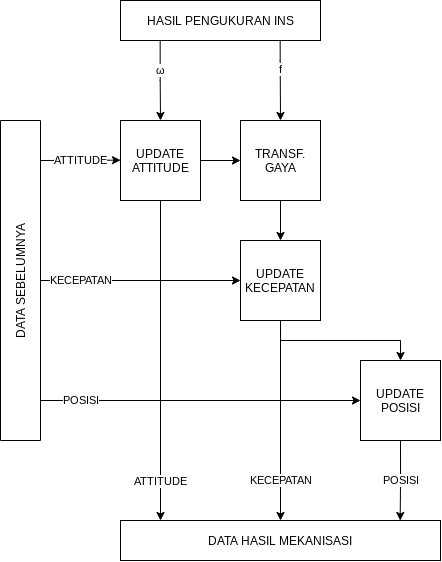
\includegraphics[width=.3\textwidth]{3-INS-mechanization.png}
    \end{center}
\end{frame}


\begin{frame}
    \frametitle{Model Data Lidar dan Kamera}
    Hasil kMeans pada deteksi Lidar berupa titik koordinat tiga dimensi dengan data berbentuk nilai centroid
    \begin{equation}
        w_{\text{lidar},i}^{t}=\left\{x_{\text{lidar}, i}^{t}, y_{\text{lidar}, i}^{t}, z_{\text{lidar},i}^{t}\right\}
    \end{equation}
    
    \vspace{2em}

    Hasil deteksi kamera berupa titik koordinat tiga dimensi dari centroid dan klasifikasi dari objek yang terdeteksi, yang tidak diproses menggunakan EKF, dan disimpan untuk penggunaan di penamaan track hasil MIPDA.
    \begin{equation}
        w_{\text{kamera},i}^{t}=\left\{x_{\text{kamera}, i}^{t}, y_{\text{kamera}, i}^{t}, z_{\text{kamera},i}^{t}\right\}
    \end{equation}
\end{frame}


\begin{frame}[allowframebreaks]
    \frametitle{Model State dan Pengukuran}
    \justifying
    $x_{j}^{t}, y_{j}^{t}, z_{j}^{t}$ merupakan posisi dari halangan relatif terhadap kendaraan, $V_{j}^{t}$ merupakan estimasi kecepatan halangan dan $\alpha_{j}^{t}$ merupakan estimasi yaw dari halangan. Vektor state $\varphi_{j}^{t}$ dapat dituliskan
    \begin{equation}
        \varphi_{j}^{t}=\left\{x_{j}^{t}, y_{j}^{t}, z_{j}^{t}, V_{j}^{t}, \alpha_{j}^{t}\right\}
    \end{equation}

    vektor pengukuran merupakan gabungan dari pengukuran posisi oleh lidar dan kamera.
    \begin{equation}
        w_{i}^{t}=\left\{x_{\text{lidar}, i}^{t}, y_{\text{lidar}, i}^{t}, z_{\text{lidar},i}^{t}, x_{\text{kamera}, i}^{t}, y_{\text{kamera}, i}^{t}, z_{\text{kamera},i}^{t}\right\}
    \end{equation}

    proses dari state dapat dituliskan
    \begin{equation}
        a_{j}^{t-1}=\left[\begin{array}{c}
        x_{j}^{t-1}+\Delta t V_{j}^{t-1} \cos \left(\alpha_{j}^{t-1}\right) \\
        x_{j}^{t-1}+\Delta t V_{j}^{t-1} \sin \left(\alpha_{j}^{t-1}\right) \\
        V_{j}^{t-1} \\
        \alpha_{j}^{t-1}
        \end{array}\right]
    \end{equation}

    matriks proses A dapat dicari dengan melakukan operasi jacobi pada $a_{j}^{t-1}$

    relasi antara vektor state dan pengukuran berbentuk persamaan nonlinier
    \begin{equation}
        w_{i}^{t}=\left[\begin{array}{c}
            x_{\text{lidar}, i}^{t}\\
            y_{\text{lidar}, i}^{t}\\
            z_{\text{lidar}, i}^{t}\\
            x_{\text{kamera}, i}^{t}\\
            y_{\text{kamera}, i}^{t}\\
            z_{\text{kamera}, i}^{t}\\
            \alpha_{i}^{t}
        \end{array}\right]^{T}=\left[\begin{array}{c}
        x_{j}^{t-1}+\Delta t V_{j}^{t-1} \cos \left(\alpha_{j}^{t-1}\right) +v_{x,j}\\
        y_{j}^{t-1}+\Delta t V_{j}^{t-1} \sin \left(\alpha_{j}^{t-1}\right)+v_{y,j}\\
        z_{j}^{t-1}+v_{z,j}\\
        x_{j}^{t-1}+\Delta t V_{j}^{t-1} \cos \left(\alpha_{j}^{t-1}\right)+v_{x,j}\\
        y_{j}^{t-1}+\Delta t V_{j}^{t-1} \sin \left(\alpha_{j}^{t-1}\right)+v_{y,j}\\
        z_{j}^{t-1}+v_{z,j}\\
        \alpha_{j}^{t-1}
        \end{array}\right]
    \end{equation} 

    dan nilai $H_j$ dapat dicari dengan menurunkan $w_{i}^{t}$
    \begin{equation}
        H_{j}^{t}=\frac{\partial h\left(w_{i}^{t}\right)}{\partial w_{i}^{t}}
    \end{equation}
\end{frame}


\begin{frame}
    \frametitle{Transformasi koordinat hasil deteksi}
    \justifying
    Sebelum masuk tahap tracking, posisi dari halangan akan ditransformasikan ke frame bumi menggunakan data posisi mobil. 
    
    Posisi kendaraan adalah vektor posisi $P = [p_x \quad p_y \quad p_z \quad \alpha \quad \beta \quad \gamma]'$, sementara itu posisi halangan adalah vektor posisi $S = [s_x \quad s_y \quad s_z]'$. Transformasi posisi halangan menjadi posisi absolut terhadap frame bumi dapat dilakukan menggunakan kombinasi matriks rotasi:

    \begin{equation}
        R(\alpha, \beta, \gamma)=
        \left(\begin{array}{ccc}
        c \alpha c \beta & c \alpha s \beta s \gamma-s \alpha c \gamma & c \alpha s \beta c \gamma+s \alpha s \gamma \\
        s \alpha c \beta & s \alpha s \beta s \gamma+c \alpha c \gamma & s \alpha s \beta c \gamma-c \alpha s \gamma \\
        -s \beta & c \beta s \gamma & c \beta c \gamma
        \end{array}\right)
    \end{equation}
    Sehingga posisi halangan terhadap frame bumi $T$ dapat dihitung dengan
    \begin{equation}
        T = R(\alpha, \beta, \gamma)S + [p_x \quad p_y \quad p_z]'
    \end{equation}
\end{frame}


\begin{frame}
    \frametitle{Hipotesa Penelitian}
    \justifying
    Dengan melakukan penggabungan beberapa sensor deteksi halangan (Lidar dan Kamera) dengan sensor deteksi posisi (INS dan GPS), diharapkan hasil tracking yang didapatkan lebih baik dibandingkan dengan tanpa melakukan penggabungan data.
\end{frame}


\begin{frame}
    \frametitle{Rencana Pengujian}
    \justifying
    Pengujian akan dilakukan untuk membuktikan hipotesa yang telah dibuat. Rencana pengujian yang akan dibuat terbagi menjadi tiga jenis pengujian:
    \begin{itemize}
        \item Pengujian hasil deteksi posisi halangan
        \item Pengujian posisi mobil
        \item Pengujian metode tracking
    \end{itemize}
\end{frame}


\begin{frame}
    \frametitle{Pengujian hasil deteksi posisi halangan}
    \justifying
    Pengujian ini dilakukan untuk menguji hasil sensor fusion kamera dengan lidar yang dihasilkan oleh EKF. Pengujian hasil deteksi posisi halangan ini akan dilakukan dengan beberapa variasi jarak dan jumlah halangan. Pada pengujian ini, akan dilakukan perbandingan metode sensor fusion pada tingkat fitur menggunakan SAF-FCOS dengan metode fusion pada tingkat data menggunakan EKF.
\end{frame}


\begin{frame}
    \frametitle{Pengujian posisi mobil}
    \justifying
    Pengujian ini dilakukan untuk menguji hasil sensor fusion dari GPS dan INS yang dihasilkan oleh IMM-EKF. Pengujian hasil deteksi posisi mobil otonom ini akan dilakukan dengan beberapa variasi lintasan, yakni:
    \begin{enumerate}
        \item lintasan lurus
        \item lintasan memutar
        \item lintasan berliku
    \end{enumerate}
\end{frame}


\begin{frame}
    \frametitle{Pengujian metode tracking}
    \justifying
    Pengujian ini dilakukan untuk menguji hasil tracking yang dihasilkan oleh metode Multi-Object Integrated Probabilistic Data Association. Pengujian hasil tracking ini akan dilakukan dengan beberapa variasi skenario, yakni:
            \begin{enumerate}
                \item tracking pada 1 objek
                \item tracking pada 2 objek
                \item skenario halangan 1 mendahului halangan 2.
                \item skenario halangan 1 berpapasan dengan halangan 2.
                \item skenario (1-4) dengan noise dan information loss pada hasil deteksi.
            \end{enumerate}
\end{frame}


\begin{frame}
    \Huge
    \begin{center}
        Rencana dan Jadwal Kegiatan
    \end{center}
\end{frame}


\begin{frame}
    \frametitle{Rencana dan Jadwal Kegiatan}
    \centering
    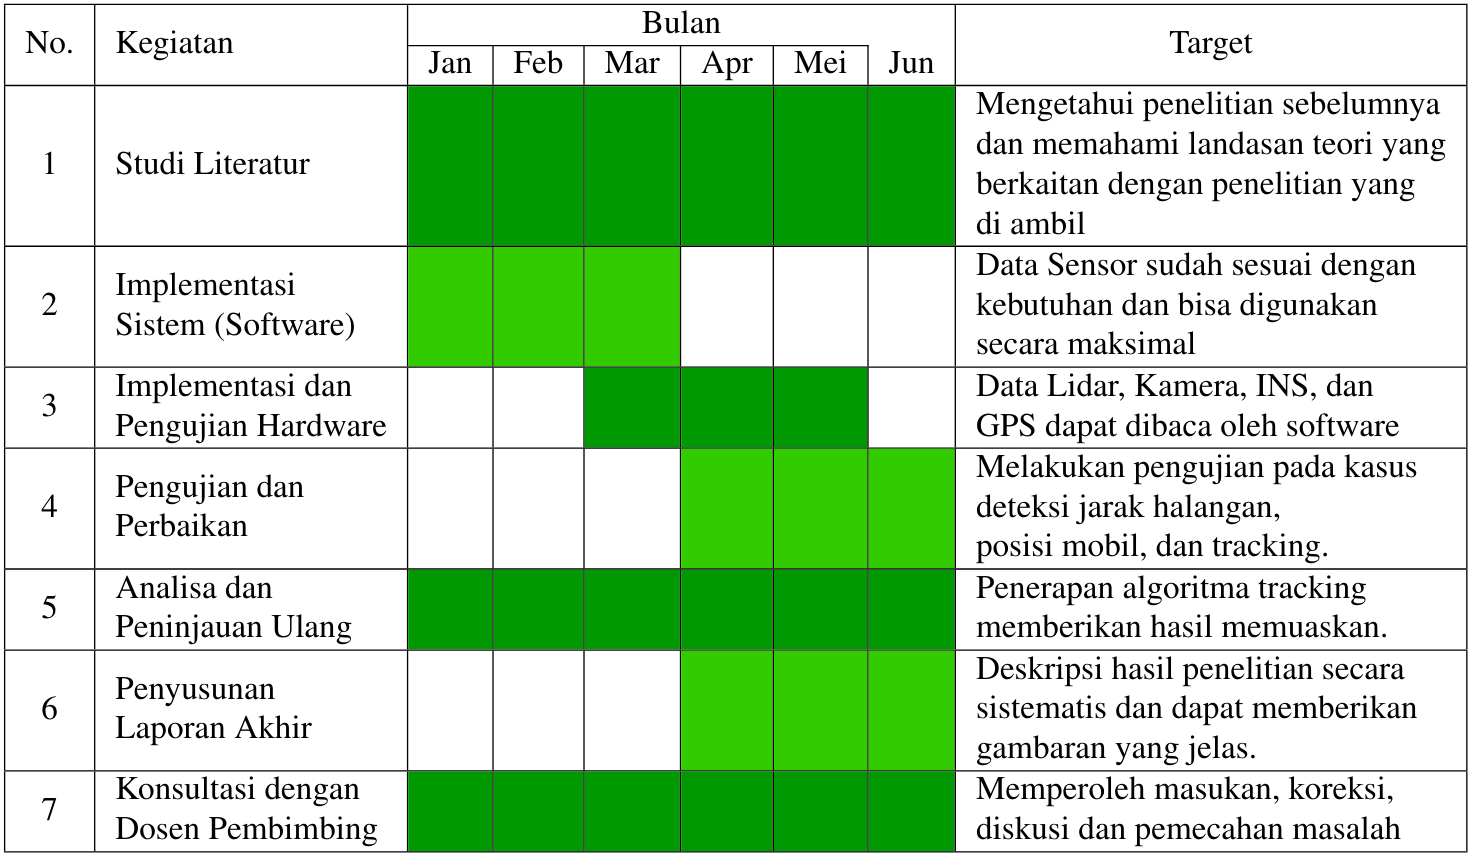
\includegraphics[width=.7\textwidth]{jadwal-v2.png}
\end{frame}

\begin{frame}
    \Huge
    \begin{center}
        Simulasi dan Pembuatan Sub-Sistem
    \end{center}
\end{frame}


\begin{frame}
    \frametitle{Pengambilan Data Lidar}
    
    Data yang dihasilkan oleh Lidar memiliki format *.bin yang tidak dapat dibaca secara langsung dan perlu diproses ke dalam bentuk kumpulan set posisi point cloud (*.pcd). Kumpulan set ini dapat ditampilkan dalam plot 3D seperti Gambar berikut

    \begin{figure}
        \centering
        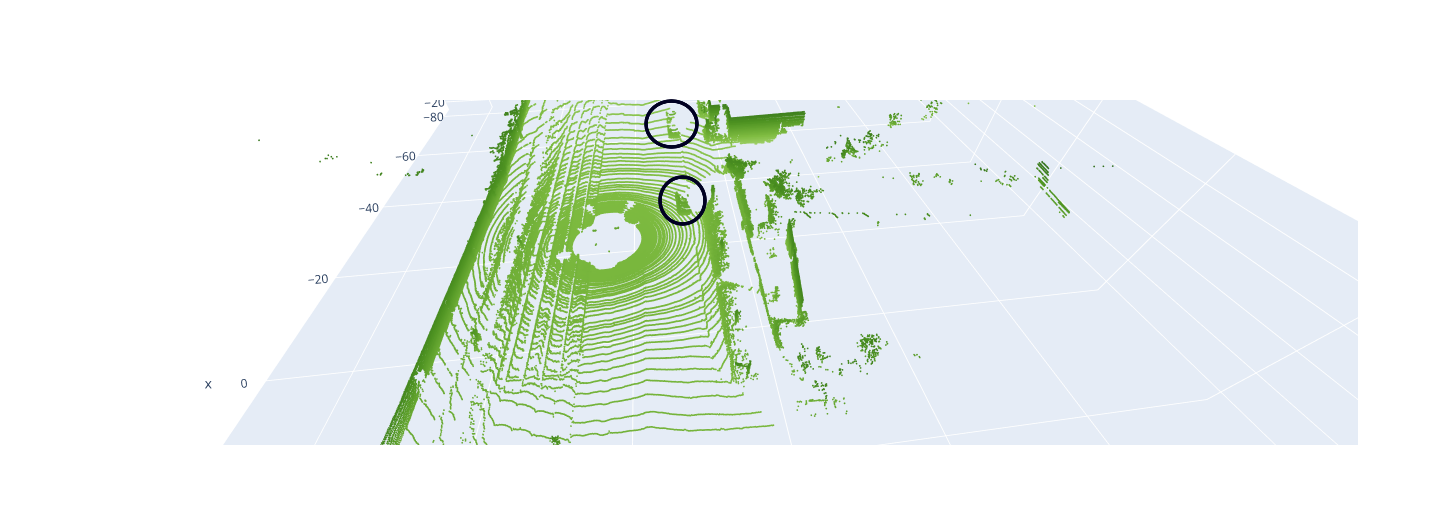
\includegraphics[width=\textwidth]{lidar-raw.png}
        \label{fig: lidar-plot3d-raw}
    \end{figure}
\end{frame}


\begin{frame}[allowframebreaks]
    \lstset{
  caption=Program konversi data *.bin Lidar menjadi \textit{list of point cloud set}, 
  label={lst: bin2pcd},
  basicstyle=\footnotesize, frame=tb,
  language=python
}
\begin{lstlisting}
def bin2pcd(binFileName):
    size_float = 4
    list_pcd = []
    with open(binFileName, "rb") as f:
        byte = f.read(size_float * 4)
        while byte:
            x, y, z, intensity = struct.unpack("ffff", byte)
            list_pcd.append([x, y, z])
            byte = f.read(size_float * 4)
    np_pcd = np.asarray(list_pcd)
    pcd = o3d.geometry.PointCloud()
    pcd.points = o3d.utility.Vector3dVector(np_pcd)
    return pcd
\end{lstlisting}
\end{frame}


\begin{frame}
    \frametitle{Lidar Clustering}
    Lidar Clustering adalah metode untuk mengelompokkan point cloud yang dihasilkan oleh lidar ke dalam cluster berdasarkan jarak eucledian antara satu titik dengan titik lainnya. Terdapat beberapa langkah yang perlu dilakukan untuk mengimplementasikan metode ini, yakni:

    \begin{itemize}
        \item Voxel Grid Processing \\
        \item Terrain Removal \\
        \item Eucledian Clustering \\
        \item Asosiasi
    \end{itemize}
\end{frame}


\begin{frame}
    \frametitle{Voxel Grid Processing}

    Data point cloud ini memiliki jumlah yang sangat banyak ($3 \times 10^5$ hingga $2 \times 10^6$ titik) sehingga akan sangat membebani algoritma clustering. Untuk mengurangi jumlah data yang digunakan, maka dapat dilakukan reduksi data point cloud dengan menggunakan metode Voxel Grid \cite{open3d_2018}. Keluaran dari metode Voxel Grid ini memiliki jumlah data yang lebih sedikit, namun tidak mengurangi kemampuan deteksi secara signifikan \cite{open3d_2018}.
    \begin{figure}
        \centering
        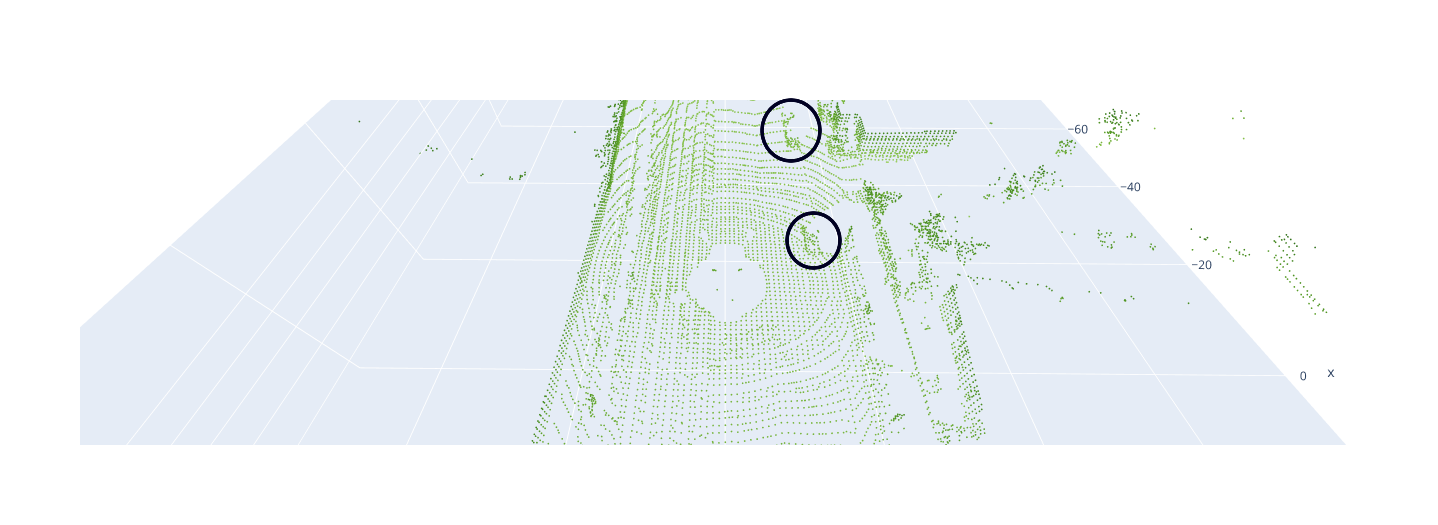
\includegraphics[width=\textwidth]{lidar-voxelize.png}
    \end{figure}
\end{frame}


\begin{frame}[allowframebreaks]
    \lstset{
  caption=Program voxel grid, 
  label={lst: voxelgrid},
  basicstyle=\footnotesize, frame=tb,
  language=python
}
\begin{lstlisting}
downpcd = pcd.voxel_down_sample(voxel_size=0.5)
o3d.visualization.draw_geometries([downpcd])
cloud_xyz = np.asarray(downpcd.points) # get xyz points
\end{lstlisting}

    Pada library Open3D telah terdapat function untuk melakukan operasi voxel grid yang dapat langsung digunakan. 
\end{frame}


\begin{frame}
    \frametitle{Terrain Removal}

    Setelah data point cloud direduksi menggunakan Voxel Grid, kita dapat menghilangkan bidang jalan dengan mencari bidang datar di sekitar lokasi $z$ minimal.Metode ini hanya efektif bila jalan berupa bidang datar.
    \begin{figure}
        \centering
        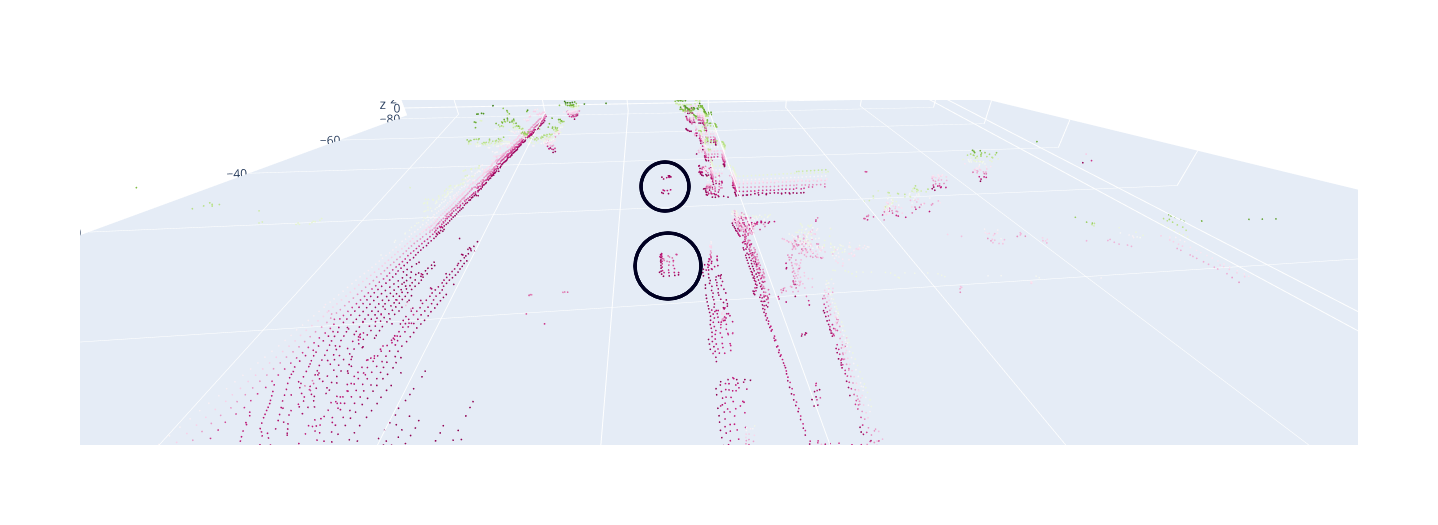
\includegraphics[width=\textwidth]{lidar-remove-floor.png}
    \end{figure}
\end{frame}


\begin{frame}[allowframebreaks]
    \lstset{
  caption=Program menghilangkan bidang jalan, 
  label={lst: removefloor},
  basicstyle=\footnotesize, frame=tb,
  language=python
}
\begin{lstlisting}
def filter_ground(cloud):
  # range antara min and max di sb-z dgn 0.1 step
  bin_range = np.arange(cloud[:,2].min(),cloud[:,2].max(), 0.1)
  # find distribution of points in z-axis
  counts, bins = np.histogram(cloud[:,2], bins = bin_range)
  # find for which z there is maximum points
  max_z = np.where(counts == max(counts))[0][0]
  # check max_z + 2 tidak overflow
  if max_z + 2 <= len(bins):
      ground_z = np.round(bins[max_z + 2], 2)
  else:
      ground_z = np.round(bins[-1], 2)
  # remove ground points
  objects_cloud = cloud[(cloud[:,2]>ground_z)]
  
  return objects_cloud, ground_z
\end{lstlisting}
\end{frame}


\begin{frame}
    \frametitle{Eucledian Clustering}

    Pada langkah ini setiap titik diiterasi untuk menghitung apakah titik ini termasuk kedalam cluster yang sama atau cluster yang berbeda.
    \begin{figure}
        \centering
        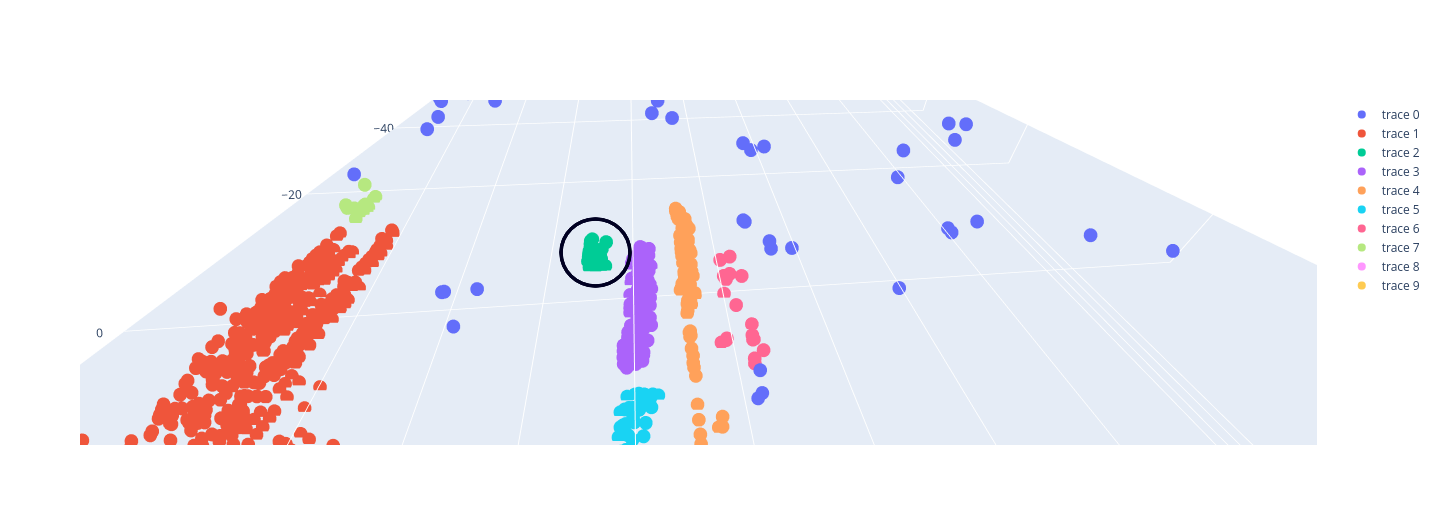
\includegraphics[width=\textwidth]{lidar-clustering.png}
    \end{figure}
\end{frame}


\begin{frame}
    \frametitle{Asosiasi}

    Langkah terakhir adalah melakukan deteksi dan penentuan bounding box pada cluster yang dianggap sebagai mobil. Langkah ini masih belum selesai dikerjakan
\end{frame}


\begin{frame}
    \frametitle{Multi-Object Tracking}

    Program Multi-Object Tracking ini terbagi kedalam dua bagian besar:
    \begin{enumerate}
        \item Filtering
        \item Track Selection
    \end{enumerate}
\end{frame}


\begin{frame}
    \frametitle{Filtering}

    Pada ujicoba ini, filtering masih menggunakan filter kalman dasar karena terdapat error pada program filtering dengan Extended Kalman Filter yang diusulkan. Model yang digunakan pada kalman filter dasar ini tidak mempertimbangkan heading kendaraan karena heading kendaraan menyebabkan nonlinearitas pada sistem yang menyebabkan kalman filter dasar tidak dapat digunakan.
\end{frame}


\begin{frame}
    \frametitle{Track Selection}

    \begin{itemize}
        \item Track merupakan object yang digunakan untuk melakukan tracking pada halangan yang terdeteksi. 
        \item Setiap track memiliki posisi awal yang diinisialisasi berdasar hasil deteksi halangan pertama. 
        \item Pada deteksi ke-2 dan seterusnya (proses update), akan dilakukan prediksi pergerakan objek menggunakan filter Kalman. 
        \item Halangan yang posisinya paling dekat ke hasil prediksi akan dianggap sebagai halangan yang sama. 
        \item Apabila halangan tidak terdeteksi, Track akan terus melakukan prediksi hingga N langkah ke depan sebelum menghapus objek Track.
    \end{itemize}
\end{frame}


\begin{frame}
    \centering
    \animategraphics[loop, autoplay, width=.5\textwidth]{24}{animasi-tracking/image}{15}{130}
\end{frame}

\begin{frame}[allowframebreaks]
    \frametitle{Referensi}
    \printbibliography
\end{frame}


\begin{frame}
    \Huge
    \begin{center}
        Terima Kasih
    \end{center}
\end{frame}


% TAMBAHAN
\begin{frame}[allowframebreaks]
    \frametitle{Pustaka 1: Tambahan}

    \begin{itemize}
        \item vektor state sistem:
        \begin{equation}
            x=\left[\begin{array}{c}
            p_{x} \\
            p_{y} \\
            v \\
            \psi \\
            \dot{\psi}
            \end{array}\right], \quad v=\sqrt{v_{x}^{2}+v_{y}^{2}}, \quad \psi=\tan ^{-1} \frac{v_{y}}{v_{x}}
            \label{eq: 2-LREKF-state}
        \end{equation}
        \item state sistem:
        \begin{equation}
            x_{k+1}=x_{k}+\left[\begin{array}{c}
            \frac{v_{k}}{\dot{\psi}_{k}}\left(\sin \left(\psi_{k}+\dot{\psi}_{k} \Delta t\right)-\sin \left(\psi_{k}\right)\right) \\
            \frac{v_{k}}{\dot{\psi}_{k}}\left(-\cos \left(\psi_{k}+\dot{\psi}_{k} \Delta t\right)+\cos \left(\psi_{k}\right)\right) \\
            0 \\
            \Delta t \\
            0
            \end{array}\right]+\nu_{k}
            \label{eq: 2-LREKF-state-eq}
        \end{equation}
        \item perhitungan prediksi $p_x$ dan $p_y$
        \begin{equation}
            \begin{array}{l}
            p_{x_{k+1}}=p_{x_{k}}+v_{k} \cos \left(\psi_{k}\right) \Delta t \\
            p_{y_{k+1}}=p_{y_{k}}+v_{k} \sin \left(\psi_{k}\right) \Delta t
            \end{array}
            \label{eq: 2-LREKF-div0}
        \end{equation}
        \item noise sistem
        \begin{equation}
            \nu_{k}=\left[\begin{array}{c}
            \frac{1}{2}(\Delta t)^{2} \cos \left(\psi_{k}\right) \nu_{a, k} \\
            \frac{1}{2}(\Delta t)^{2} \sin \left(\psi_{k}\right) \nu_{a, k} \\
            \Delta t \nu_{a, k} \\
            \frac{1}{2}(\Delta t)^{2} \nu_{\ddot{\psi}, k} \\
            \Delta t \nu_{\ddot{\psi}, k}
            \end{array}\right]
            \label{eq: 2-LREKF-state-noise}
        \end{equation}
        \item kovarian
        \begin{equation}
            Q=\left[\begin{array}{ccccc}
                \frac{\Delta t^{4}}{4} \sigma_{a_{x}}^{2} & 0 & \frac{\Delta t^{3}}{2} \sigma_{a_{x}}^{2} & 0 & 0 \\
                0 & \frac{\Delta t^{4}}{4} \sigma_{a_{y}}^{2} & \frac{\Delta t^{3}}{2} \sigma_{a_{y}}^{2} & 0 & 0 \\
                \frac{\Delta t^{3}}{2} \sigma_{a_{x}}^{2} & \frac{\Delta t^{3}}{2} \sigma_{a_{y}}^{2} & \Delta t^{2} \sigma_{a}^{2} & 0 & 0 \\
                0 & 0 & 0 & \Delta t^{2} \sigma_{\psi}^{2} & 0 \\
                0 & 0 & 0 & 0 & \Delta t^{2} \sigma_{\dot{\psi}}^{2}
                \label{eq: 2-LREKF-state-cov}
            \end{array}\right]
        \end{equation}
        \item matriks pengukuran dan error pengukuran Lidar
        \begin{equation}
            \begin{array}{l}
            H_{\text {lidar }}=\left[\begin{array}{lllll}
            1 & 0 & 0 & 0 & 0 \\
            0 & 1 & 0 & 0 & 0
            \end{array}\right], \\
            R_{\text {lidar }}=E\left[\omega \omega^{\top}\right]=\left[\begin{array}{cc}
            \sigma_{p_{x}}^{2} & 0 \\
            0 & \sigma_{p_{y}}^{2}
            \end{array}\right],
            \end{array}
            \label{eq: 2-LREKF-HQ}
        \end{equation}
        \item matriks pengukuran dan error pengukuran Radar
        \begin{equation}
            H_{j_{\mathrm{radar}}}=\frac{1}{|p|^{2}}\left[\begin{array}{cccc}
            p_{x}|p| & p_{y}|p| & 0 & 0 \\
            -p_{y} & p_{x} & 0 & 0 \\
            \frac{p_{y} v p_{1}}{|p|} & -\frac{p_{x} v p_{1}}{|p|} & p_{2}|p| & v p_{1}|p|
            \end{array}\right]
        \end{equation}
        $$
        |p|=\sqrt{p_{x}^{2}+p_{y}^{2}}
        $$
        $$
        p_{1}=p_{y} \cos (\psi)-p_{x} \sin (\psi)
        $$
        $$
        p_{2}=p_{x} \cos (\psi)+p_{y} \sin (\psi)
        $$
        \begin{equation}
            R_{\text {radar }}=\left[\begin{array}{ccc}
            \sigma_{p}^{2} & 0 & 0 \\
            0 & \sigma_{\varphi}^{2} & 0 \\
            0 & 0 & \sigma_{\dot{\rho}}^{2}
            \end{array}\right]
        \end{equation}
    \end{itemize}

\end{frame}
\begin{frame}[allowframebreaks]
    \frametitle{Pustaka 2: Tambahan}
    \justifying

    Block Radar dan Kamera:\\
    Blok radar dan kamera adalah ResNet-50 yang dimodifikasi. Blok ini memiliki dua blok konvolusi, yakni blok \textit{R-Stem} dan \textit{R-Block1}. \textit{R-Stem} adalah modul stem asli ResNet-50 untuk memproses data masukan dari sensor. R-Block1 mirip dengan tahap pertama dari ResNet-50, tetapi hanya memiliki blok residual.

    Ukuran konvolusi SAF:\\
    SAF yang paper ini usulkan terdiri dari tiga kelompok lapisan konvolusi untuk mengekstrak matriks spatial attention. Konfigurasi dalam layer "Conv $1 \times 1$" berarti ukuran kernel $1 \times 1 \times 256 \times 1$, stride $(1, 1)$, padding $[0, 0]$. Adapun lapisan "Conv $3 \times 3$" dan "Conv $5 \times 5$" konfigurasinya masing-masing
    $$
        \{3 \times 3 \times 256 \times 1, (1, 1), [1, 1]\}
        \quad dan \quad
        \{5 \times 5 \times 256 \times 1, (1, 1), [2, 2]\}
    $$

    Block RetinaNet:\\
    loss functionnya
    \begin{equation}
        L\left(c_{i}, t_{i}\right)=1 / N_{p o s} \sum_{i} L_{c l s}\left(c_{i}, c_{i^{*}}\right)+\frac{\lambda}{N_{p a s}} \sum_{i} I_{c_{i}>0} L_{r e g}\left(t_{i}, t_{i^{*}}\right)
        \label{eq: FCOS-loss-fn}
    \end{equation}

    \begin{center}        
        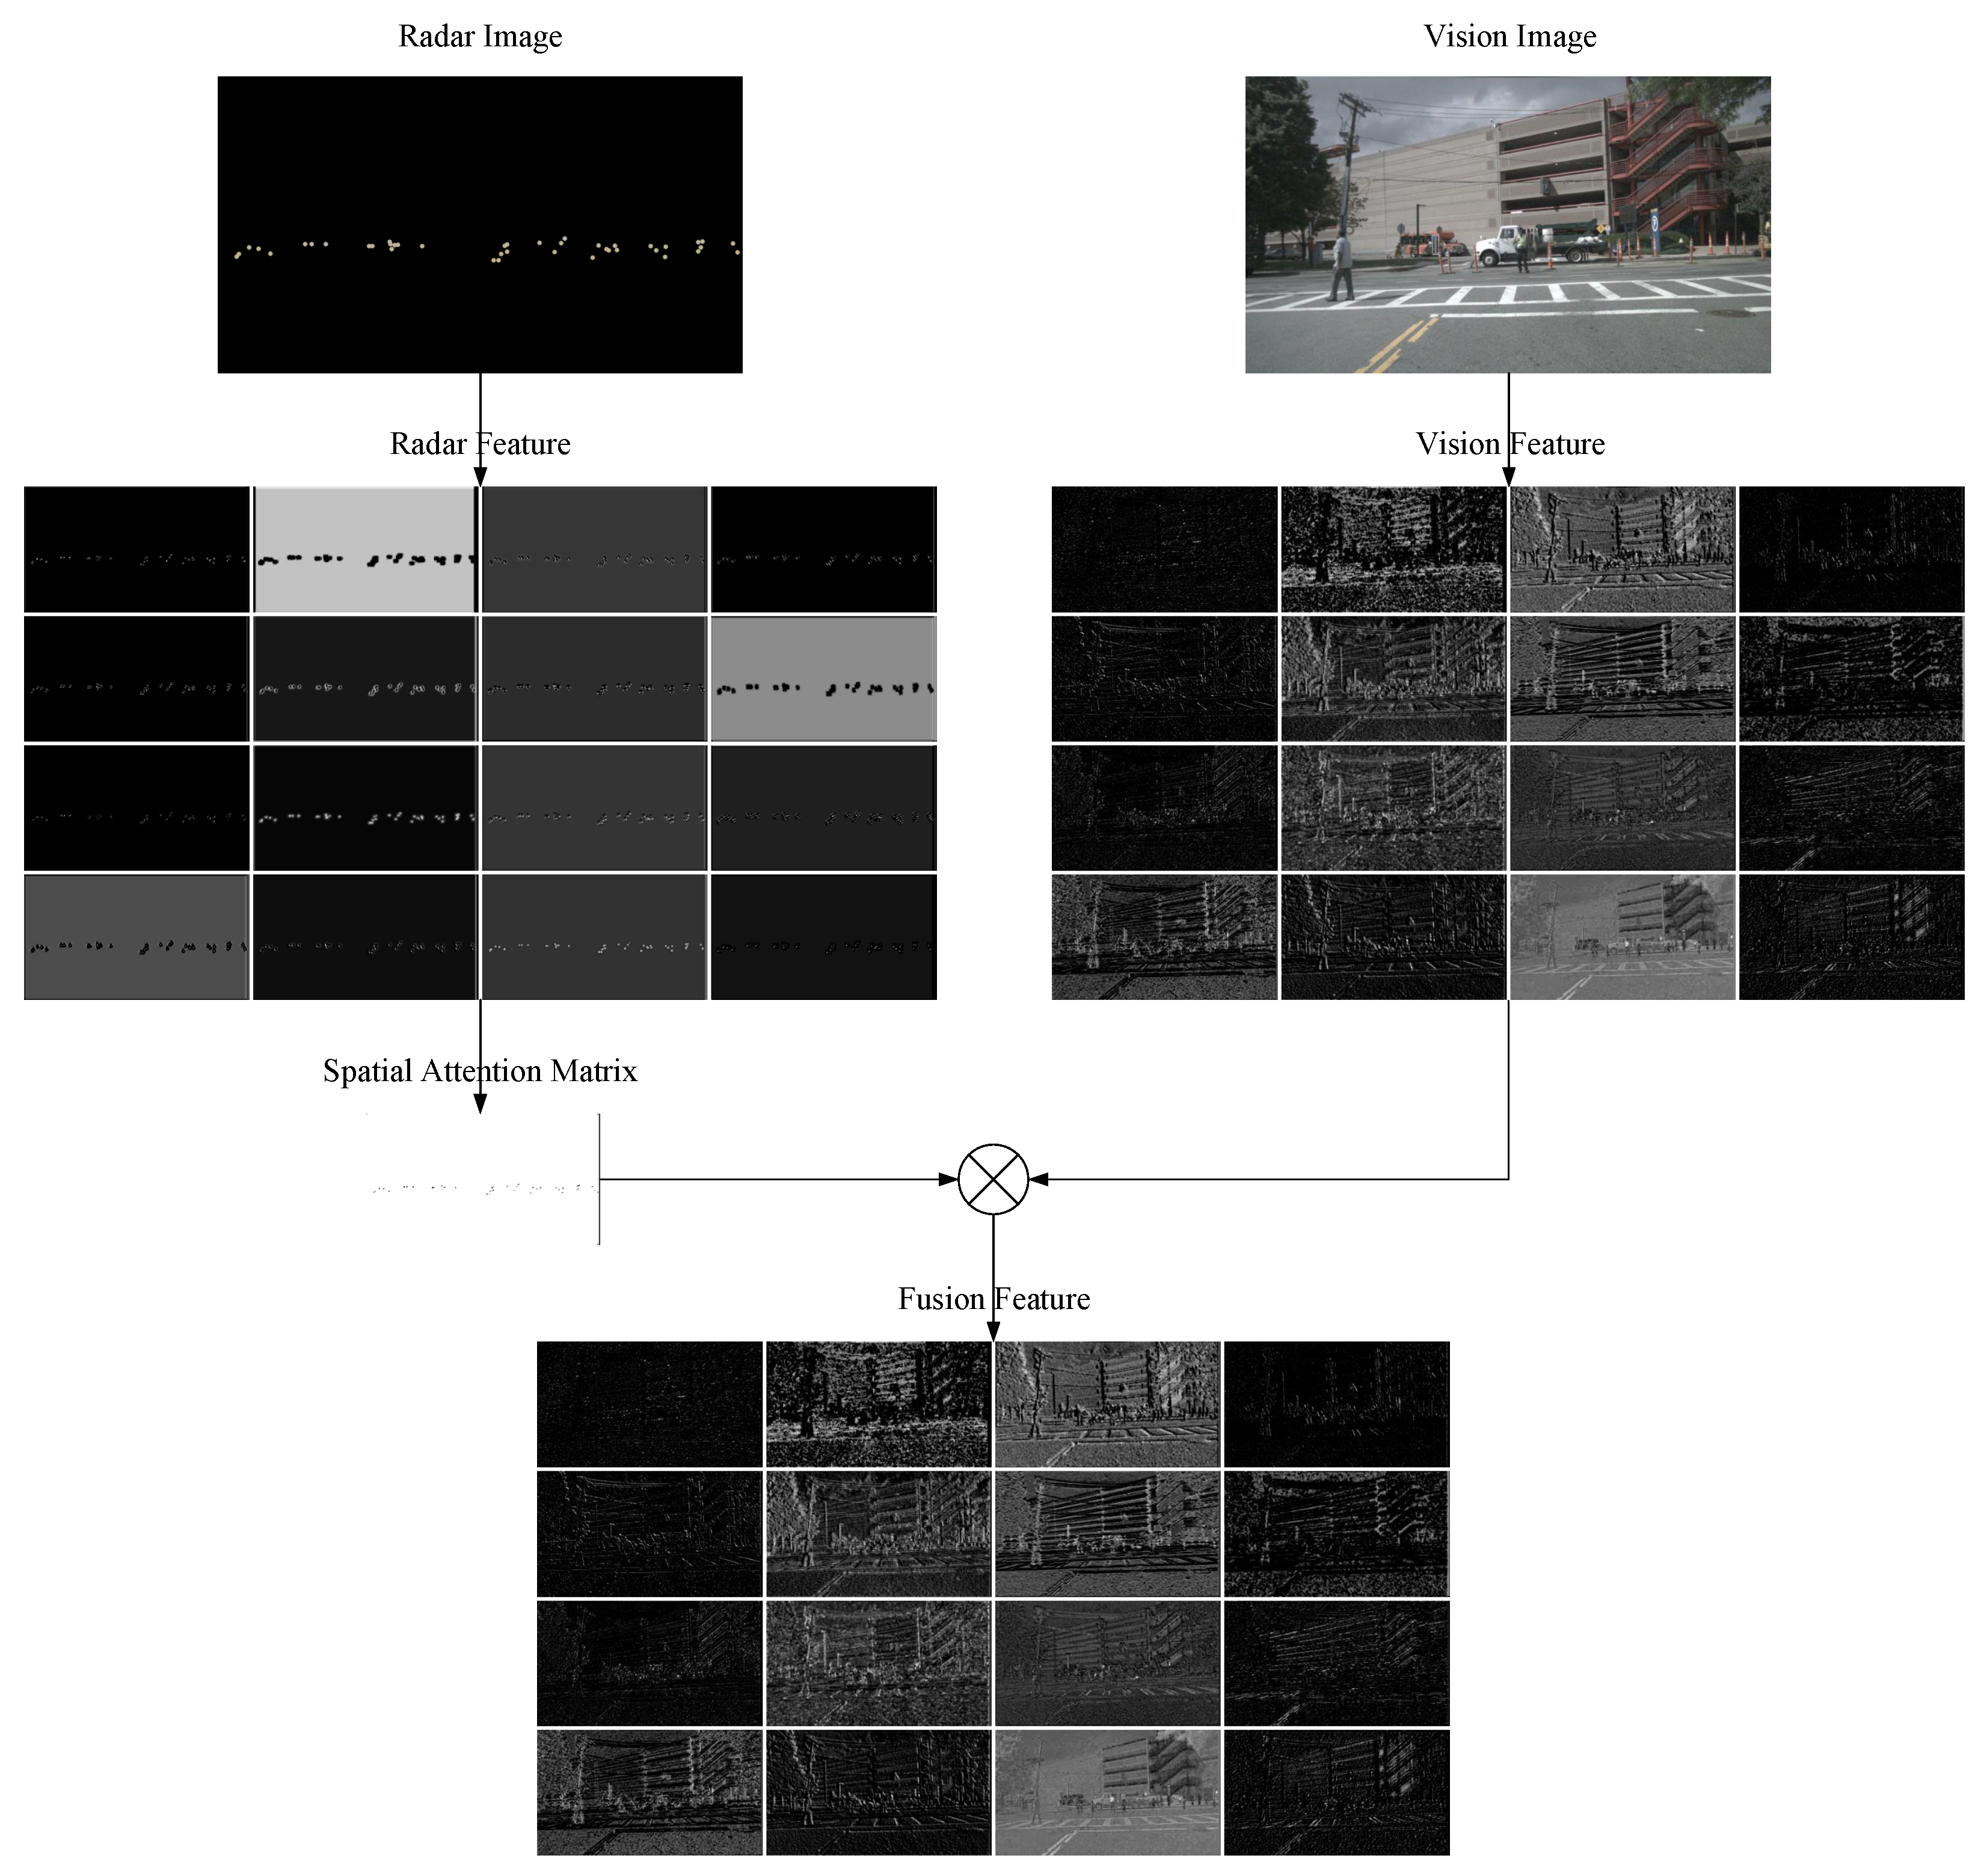
\includegraphics[width=.45\textwidth]{2-SAF-feature.png}
    \end{center}

\end{frame}
\begin{frame}[allowframebreaks]
    \frametitle{Pustaka 3: Wavelet Denoising}
    \justifying

    Fungsi threshold dari wavelet denoising ini terdiri dari dua macam, yakni soft threshold dan hard threshold.
    \begin{equation}
        \hat{d}=\left\{\begin{array}{ll}
        d, & |d| \geq \lambda \\
        0, & |d|<\lambda
        \end{array}\right.
        \label{eq: 2-GPSINS-WD-hard-thres}
    \end{equation}
    \begin{equation}
        \hat{d}=\left\{\begin{array}{ll}
        sgn(d)(|d|-\lambda), & |d| \geq \lambda \\
        0, & |d|<\lambda
        \end{array}\right.
        \label{eq: 2-GPSINS-WD-soft-thres}
    \end{equation}
    dimana $d$ merupakan koefisien wavelet yang belum diproses, dan $\hat{d}$ merupakan koefisien wavelet setelah dilakukan thresholding. 
    
    Threshold dari $\lambda$ adalah
    \begin{equation}
        sgn(x)=\left\{\begin{array}{ll}
        1, & x>0 \\
        0, & x=0 \\
        -1, & x<0
        \end{array}\right.
    \end{equation}
    \begin{equation}
        \lambda=\underset{T>0}{\arg }\left\{\min \left[\sum_{i=0}^{N}\left(\left|d_{i}\right| \wedge \lambda\right)^{2}+N \sigma_{n}^{2}-2 \sigma_{n}^{2} \sum_{i=0}^{N} I\left(|d_{i}|<\lambda\right)\right]\right\}
        \label{eq: 2-GPSINS-WD-lambda}
    \end{equation}
    \begin{equation}
        I(x)=\left\{\begin{array}{ll}
        1, & \text { true } \\
        0, & \text { false }
        \end{array}\right.
    \end{equation}
\end{frame}

\end{document}